\section{Aufgabe 1}
\subsection{Aufgabe 1 a)}
Die initiale Spotbreite des Protonenstrahls bestimmt sich aus der \enquote{FWHM} größe, die durch python Methoden abgelesen werden kann.
Hierfür wurde eine Maske erstellt mit einer Epsilonumgebung von $0.01$ und
\begin{verbatim}
    eps = 0.01
    mask1 = np.asarray(task1[:,3] > 0.5-eps)
    mask2 = np.asarray(task1[:,3] < 0.5+eps).
\end{verbatim}
Die gefunden boolean Werte werden anschließend auf den gegeben Array angewandt wobei die Resultate bei $-1.05$ und $1.0$ eine Spotbreite von \SI{2.05}{\cm} geben.
\begin{figure}
    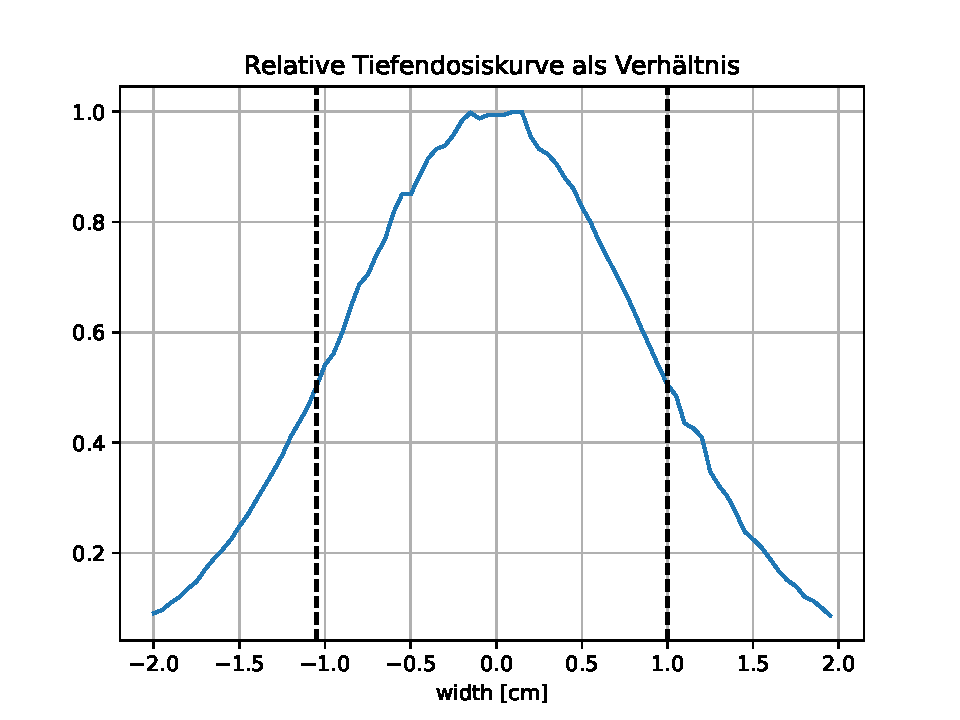
\includegraphics[width = 0.8\textwidth]{../poject/task1/task1a.pdf}
\end{figure}

\subsection{Aufgabe 1 b)}

